\documentclass[border=8pt]{standalone}
\usepackage{tikz}
\usetikzlibrary{positioning,arrows.meta,calc}
\begin{document}
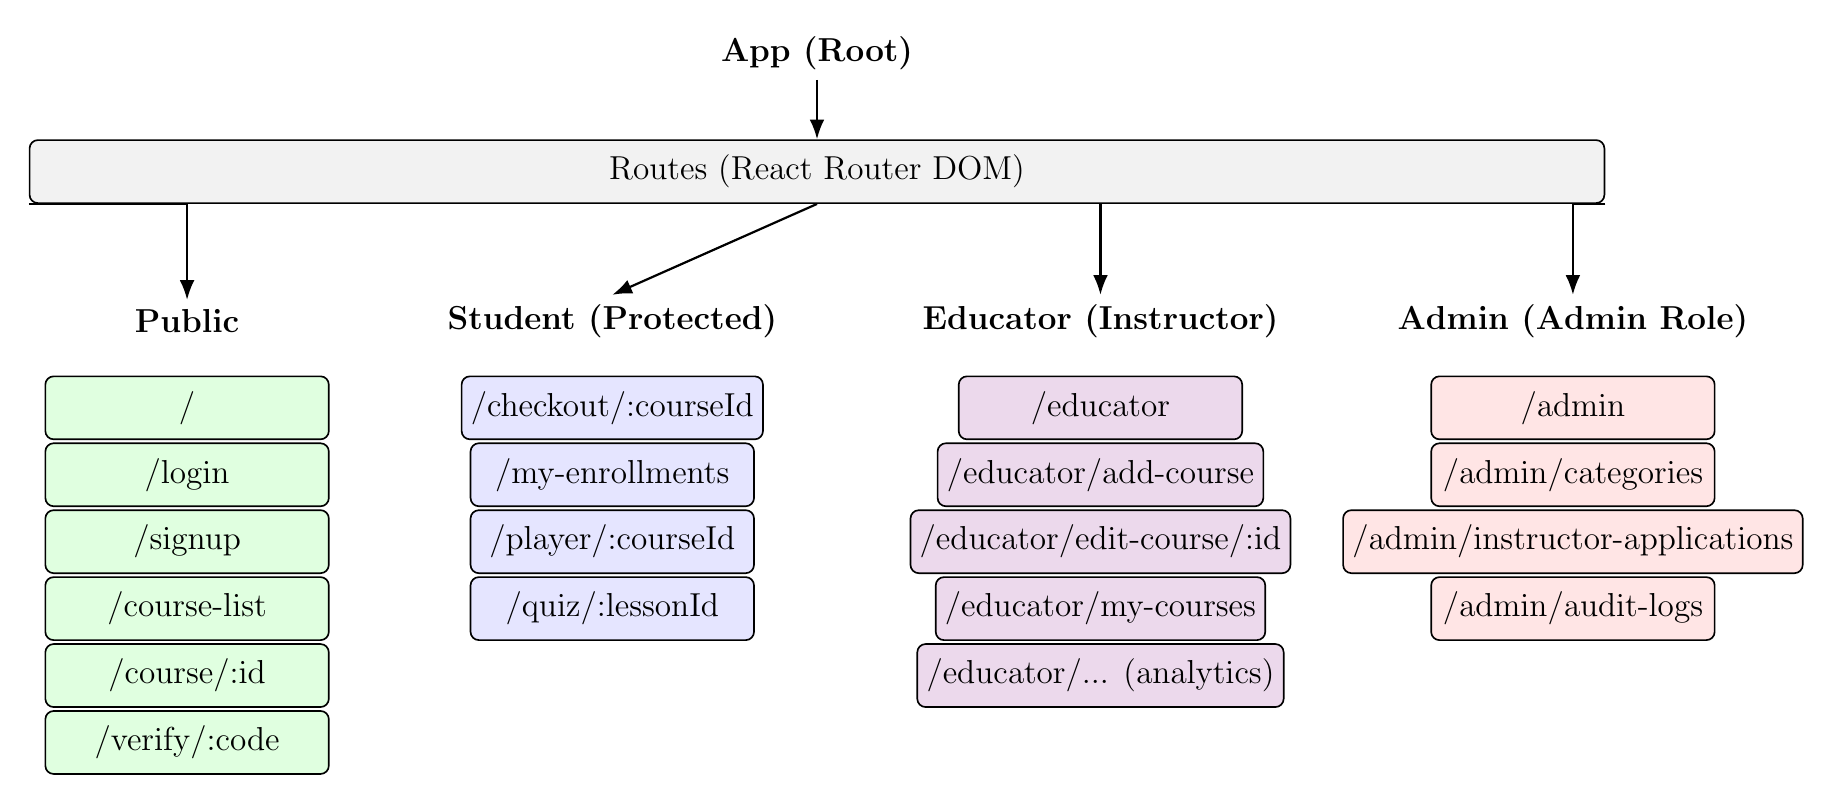
\begin{tikzpicture}[
  font=\large,
  arr/.style={-{Latex[length=2.5mm]}, line width=0.8pt},
  cat/.style={font=\bfseries\large},
  route/.style={rounded corners=3pt, draw=black, line width=0.6pt, minimum width=3.6cm, minimum height=0.8cm, align=center, fill=white}
]

\node[cat] (root) at (0,9) {App (Root)};
\node[route, minimum width=20cm, fill=gray!10] (routes) at (0,7.5) {Routes (React Router DOM)};
\draw[arr] (root) -- (routes.north);

% Category labels
\node[cat] (pub)  at (-8.0,5.6) {Public};
\node[cat] (stu)  at (-2.6,5.6) {Student (Protected)};
\node[cat] (edu)  at (3.6,5.6) {Educator (Instructor)};
\node[cat] (adm)  at (9.6,5.6) {Admin (Admin Role)};

\draw[arr] (routes.south west) -| (pub.north);
\draw[arr] (routes.south) -- (stu.north);
\draw[arr] ($(routes.south)+(3.6,0)$) -| (edu.north);
\draw[arr] (routes.south east) -| (adm.north);

% Public routes (green) - no auth required
\node[route, fill=green!12] (p1) at ($(pub)+(0,-1.1)$)  {/};
\node[route, fill=green!12] (p2) at ($(p1)+(0,-0.85)$)  {/login};
\node[route, fill=green!12] (p3) at ($(p2)+(0,-0.85)$)  {/signup};
\node[route, fill=green!12] (p4) at ($(p3)+(0,-0.85)$)  {/course-list};
\node[route, fill=green!12] (p5) at ($(p4)+(0,-0.85)$)  {/course/:id};
\node[route, fill=green!12] (p6) at ($(p5)+(0,-0.85)$)  {/verify/:code};

% Student routes (blue) - any authenticated role
\node[route, fill=blue!10] (s1) at ($(stu)+(0,-1.1)$)  {/checkout/:courseId};
\node[route, fill=blue!10] (s2) at ($(s1)+(0,-0.85)$)  {/my-enrollments};
\node[route, fill=blue!10] (s3) at ($(s2)+(0,-0.85)$)  {/player/:courseId};
\node[route, fill=blue!10] (s4) at ($(s3)+(0,-0.85)$)  {/quiz/:lessonId};

% Educator routes (purple) - INSTRUCTOR or ADMIN role
\node[route, fill=violet!15] (e1) at ($(edu)+(0,-1.1)$)  {/educator};
\node[route, fill=violet!15] (e2) at ($(e1)+(0,-0.85)$)  {/educator/add-course};
\node[route, fill=violet!15] (e3) at ($(e2)+(0,-0.85)$)  {/educator/edit-course/:id};
\node[route, fill=violet!15] (e4) at ($(e3)+(0,-0.85)$)  {/educator/my-courses};
\node[route, fill=violet!15] (e5) at ($(e4)+(0,-0.85)$)  {/educator/... (analytics)};

% Admin routes (red) - ADMIN role only
\node[route, fill=red!10] (a1) at ($(adm)+(0,-1.1)$)  {/admin};
\node[route, fill=red!10] (a2) at ($(a1)+(0,-0.85)$)  {/admin/categories};
\node[route, fill=red!10] (a3) at ($(a2)+(0,-0.85)$)  {/admin/instructor-applications};
\node[route, fill=red!10] (a4) at ($(a3)+(0,-0.85)$)  {/admin/audit-logs};

\end{tikzpicture}
\end{document}
